\providecommand{\main}{./report}
\documentclass[../main.tex]{subfiles}
\begin{document}


\section{Evaluating Feature Rankings}\label{section:evaluation}
Like seen in Chapter~\ref{section:related-work}, the evaluation of feature- ranking and selection methods is a nontrivial process, that has been conducted in many ways in the literature. Because of this reason, it is desired to acquire a general evaluation method that is applicable to all feature- ranking and selection methods - which is argued for to be a solid and scientifically sound evaluation process. In this chapter, a reasoning is given on which evaluation metrics are possibly sensible to use, after which a general recommendation on evaluation for different scenarios is given.



\subsection{Cross-Validation and Bootstrapping}\label{section:cv}
Several steps can be undertaken to provide more reliable estimates of the feature ranker performance. The goal is to prevent the practitioner to get promising but misleading results, whilst keeping the performance of the benchmarking process at a reasonable level.



\subsubsection{Cross-Validation}
% why CV
For almost any Machine Learning experiment, it is recommended to use some form of \gls{cv}. Because a model has the possibility to get `learn' the training data, evaluating the performance of an estimator on just the set of training data is dangerous practice. Evaluation metrics can be misleading, suggesting better model performance than is actually the case - when such a model is employed outside the realm of the training data, model generalization performance can turn out to be very poor. Thus, also in the context of benchmarking feature- ranking and selection algorithms, validation must be performed by holding out a set of the available data samples at hand.

% 5-fold and 10-fold cv
The most simple form of \gls{cv} is a training/testing split, in which the practitioner holds out one set of the example data for use in the testing phase - it is to be remain unseen by the model during the training phase. More robust methods include training the model multiple times on various training datasets and evaluating on the held out testing data. This can be done using 5-fold or 10-fold \gls{cv}, where, for example, in the case of 5-fold \gls{cv} \sfrac{4}{5}th of the data is reserved for training and \sfrac{1}{5}th for testing, repeated for each fold - so 5 times.

% beware: perform cv correctly
What is especially important in the process of conducting \gls{cv}, is that no operations are performed \textbf{before} having split the data, that can influence the experimental results. For example, in the scenario where one want to select variables to be included in some feature subset and run some prediction estimators afterward, a practitioner must be careful to split the data before the variable selection process. This is because otherwise, the predictive estimators might gain an unfair advantage due to having already seen the left out samples, i.e. they have already gained an advantage from the variable selection that was performed on the full dataset. This might cause skewed and misleading estimations of the error rate of the estimators - causing faulty models. Therefore, it is at all times important to keep in mind the `right' way of performing \gls{cv}: split first before running any operations that regard the dataset samples \citep{ambroise_selection_2002}.




\subsubsection{Bootstrapping}\label{section:bootstrapping}
% bootstrapping
Bootstrapping, on the other hand, is a similar but different process. Performing a bootstrap is a classical method for estimating statistical quantities regarding the learning process, such as variance, prediction error, or bias. The process works by resampling the dataset with replacement $B$ times, such to create $B$ different permutations of the dataset. Then, the learning process is repeated for each of the $B$ bootstrap datasets, i.e., refitting the estimators for each of the permuted datasets. If, for example, the designated dataset is denoted like $\mathbf{Z}=\left(z_{1}, z_{2}, \ldots, z_{b}\right)$ with each sample $z_{i}=\left(x_{i}, y_{i}\right)$, then the $b$-th bootstrap permutation of the dataset can be denoted as $\mathbf{Z}^{* b}$. Such, estimates can be made of, for example, the variance of some statistical quantity $S$ computed over the dataset $\mathbf{Z}$:

\begin{equation}\label{eq:variance-bootstrap}
\widehat{\operatorname{Var}}[S(\mathbf{Z})]=\frac{1}{B-1} \sum_{b=1}^{B}\left(S\left(\mathbf{Z}^{* b}\right)-\bar{S}^{*}\right)^{2},
\end{equation}

which can be seen to be the unbiased average of the statistical quantity $S$ over the $B$ bootstrap permutations of $\mathbf{Z}$. Note that the average value of the statistic $S$ is computed like so:

\begin{equation}\label{eq:average-bootstrap}
\bar{S}^{*}=\sum_{b} S\left(\mathbf{Z}^{* b}\right) / B,
\end{equation}

i.e. by averaging $S$ over the $B$ bootstraps. Like such, a reasonable estimate can be made of any statistical quantity computed over the dataset, as long as the quantity can be computed for any permutation on the dataset and enough computational resources are available to run $B$ repeated experiments on each of the permutations.

% bootstrapping for feature ranking
The practice of bootstrapping comes useful to the evaluation of feature- ranking and selection algorithms, allowing the practitioner to better estimate quantities that would previously be less reliable estimates. Examples of such quantities are the feature ranking algorithm stability, variance, or fitting time. Especially in assessing the algorithm stability, there exists an interest to know how the designated algorithm functions under conditions of varying samples. For this, bootstrapping is especially useful, since the exact data generating distribution at hand is often not available- meaning no more samples can be drawn from the distribution to generate a larger data population. In the lack of a data generating distribution, resampling with replacement offers a solution.




\subsection{Validation estimators}\label{section:evaluation-validation-estimators}
% validation estimators: how they work
A straight-forward way to evaluate the performance of a feature selection algorithm is to run the ranking algorithm, and subsequently run a `validation' estimator on the selected feature subset. The quality of the selected feature subset is then quantified through the performance of the validation estimator: when more informative and relevant features are selected, validation estimator performance presumably goes up. The validation estimator can be configured to be any classifier or regressor, dependent on the prediction task at hand, though often choices are made from a common set of estimators as can be seen in Table~\ref{table:evaluation-metrics-table}. 

% feature rankings
This idea can be extended to feature rankings. Many feature selection algorithms are in fact feature ranking algorithms and do not provide a built-in mechanism to perform feature subset selection - the algorithms allow a user to define the desired amount of features to be selected using a hyper-parameter, which then uses its feature ranking internally to construct a feature subset, like explained in Section~\ref{section:methods-ranking-types}. It is therefore desired to also benchmark such algorithms in a systematic way: allowing more flexibility with respect to the evaluation process.

\begin{figure}[ht]
    \centering
    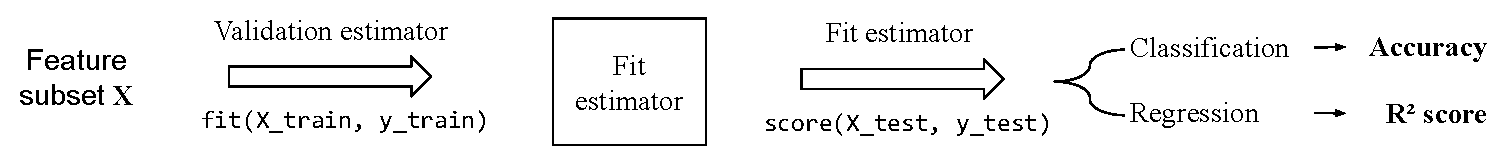
\includegraphics[width=\linewidth]{report/images/schematic-validation-estimators.pdf}
    \caption{The process of running a validation estimator on a feature subset. In the case of a feature ranking, a validation estimator is fit for some various amount of feature subsets. Often, feature subsets with some number of the highest ranked features are evaluated.}
    \label{fig:schematic-validation-estimators}
\end{figure}

As can be seen in Figure~\ref{fig:schematic-validation-estimators}, the process of running a validation estimator is straight-forward. Once a feature subset has been determined by thresholding a feature ranking or using the feature subset computed by a feature selection algorithm, a validation estimator is trained and evaluated on the held-out test set. Afterwards, a suitable evaluation metric is used depending on the learning task at hand: classification or regression (note the \hyperref[section:introduction]{research scope} was confined to just these two tasks). Exactly how many validation estimators are fit to evaluate a feature ranking depends on the ranking type (Section~\ref{section:methods-ranking-types}). In the case of a feature support vector, only the feature subset might have to be evaluated, whilst for feature- importance or ranking vectors one might want to evaluate the first $k$ best feature subsets. Generally, each of the vectors are evaluated like so:

\begin{itemize}
    \item Feature importance vector (Section~\ref{section:feature-importance-definition}). Fit $k$ validation estimators, for the first $k$ best feature subsets, starting with a feature subset including only the highest ranked feature and subsequently including lower-ranked features. $k$ might be chosen depending on the dataset size at hand.
    \item Feature support vector (Section~\ref{section:feature-support-definition}). A feature subset was already selected by the feature selection algorithm and such the feature subset can be directly evaluated by the validation estimator.
    \item Feature ranking vector (Section~\ref{section:feature-rankings-definition}). A feature ranking can fit $k$ validation estimators; similarly to the feature importance vector.
\end{itemize}

Notably, in the case where a feature ranking algorithm supports computing both feature- importance or ranking vectors and the feature subset, i.e., the feature support vector, simply the $k$ best feature subsets can be evaluated by the validation estimator - assuming the selected feature subset to be included in one of the $k$ best feature subsets. If for some reason the selected feature subset $\hat{\mathbb{S}}$ is not in any of the $k$ best feature subsets, it will still be evaluated by a validation estimator separately.

A bootstrap can be used to generate more accurate estimations of the validation process. Especially for validation estimators that are sensible to varying permutations of the training data this process is useful - since otherwise validation metrics could be particularly misleading. In this way, given either an accuracy- or R\textsuperscript{2} score for classification and regression, respectively, an averaged bootstrapped score can be computed. This is done simply by plugging in either the R\textsuperscript{2} score or accuracy (or any other metric suitable for regression- or classification) into Equation~\ref{eq:average-bootstrap}.





\subsection{Apriori knowledge on relevant features}\label{section:evaluation-apriori-knowledge}
% how to retrieve apriori info
In the scenario where we know \textit{\gls{apriori}} which features are relevant, more direct evaluation can be applied on the constructed feature ranking. Such apriori ground-truth information can be gained in a couple of ways: (1) by utilising human domain expert knowledge, (2) by augmenting real-world datasets with noisy dimensions and assuming all other dimension to be uniformly relevant or lastly (3) by generating synthetic datasets with known feature importance levels (see Section~\ref{section:pipeline-components-datasets}. In the context of this section, the assumption is made that the feature importance scores are simply `known' apriori: no restriction is made on exactly how feature relevance ground truth was retrieved.

% why its better
Knowing the relevant dataset features apriori can be useful information to the feature ranking evaluation process. This is because even though the goal of feature- ranking and selection algorithms is to separate the useful from the irrelevant features, the performance of such a ranking is nowadays most commonly evaluated by training yet another estimator; the `validation' estimator (Section~\ref{section:related-work} and Section~\ref{section:evaluation-validation-estimators}). This makes the evaluation scores dependent on the validation estimator, requiring publications to have run the same validation estimator to make the results comparable between papers. Also, for some datasets, the chosen validation estimator might be sophisticated enough to make up for any noisy dimensions that were added - reducing the differences between the feature rankings, which is instead desired to be amplified to determine which feature ranker is the best for which dataset. Lastly, a sophisticated validation estimator might also perform a form of feature selection on its own, which might also skew the performance of faulty feature rankings that included lots of noisy dimensions in its feature subset. For these reasons, it is interesting to investigate the possibilities to find robust and reliable evaluation methods that do not require a validation estimator.

% evaluation using the ground-truth
Using the ground-truth relevant features, an accompanying evaluation metric can be constructed. Taking into consideration how different feature ranking algorithms construct various types of feature rankings as described in Section~\ref{section:methods-ranking-types}, a suitable metric can be created for each.

% feature importance
\textbf{Feature importance} (Section~\ref{section:feature-importance-definition}) scores are defined to be a real-valued $p$ dimensional vector, $\hat{\boldsymbol{w}}$. In order to evaluate the closeness of the vector $\hat{\boldsymbol{w}}$ to the dataset ground truth $\boldsymbol{w}$, a range of metrics can be used. A first approach would be to regard the estimated vector as an estimation of a continuous target vector, i.e., to regard the problem as a regression type of task. In such a perspective, each predicted feature importance would pose as a data sample. In this way, usual metrics related to the regression task can be used.

The \textbf{R\textsuperscript{2}-score} is one such metric that can be used in this context. This can be formalized like so:

\begin{equation}
\begin{aligned}
R^{2}&=1-\frac{\mathrm{RSS}}{\mathrm{TSS}} \\
\text{where}&\\
\mathrm{RSS} &= \sum_{i=1}^{n}\left(y_{i}-f\left(x_{i}\right)\right)^{2} =\sum_{i=1}^{p}\left(w_i - \hat{w_i} \right)^{2}, \text{ and}\\
\mathrm{TSS} &= \sum_{i=1}^{n}\left(y_{i}-\bar{y}\right)^{2} =\sum_{i=1}^{p}\left( w_i - \bar{\boldsymbol{w}} \right)^{2}, \\
\end{aligned}
\end{equation}

which can be used to evaluate the closeness of the predicted feature importance vector $\hat{\boldsymbol{w}}$ to the ground-truth feature importance vector $\boldsymbol{w}$.

The \textbf{logistic-loss}, or \textit{cross-entropy} score is another metric which can be employed to quantify the quality of a feature importance vector $\hat{\boldsymbol{w}}$. In this scenario, however, the target variables are regarded to be binary labels, which therefore means the predicted feature importance vector $\hat{\boldsymbol{w}}$ is to be compared against $\boldsymbol{s}$ instead of $\boldsymbol{w}$. Remember, from Section~\ref{section:feature-support-definition}, that $\boldsymbol{s}$ is the $p$-dimensional vector indicating with a boolean whether or not the feature is relevant, i.e. $\boldsymbol{s} \in \mathbb{B}^p$. Such, a zero indicates a feature is not relevant; and a one indicates the feature is informative or relevant. In this way, a feature ranker approximates the true binary relevance labels $\boldsymbol{s}$ with probability values arranged in the probability vector $\hat{\boldsymbol{w}}$. The logistic loss can be formalized like so:

\begin{equation}
\begin{aligned}
L_{\log }(y, p) &= -\log \operatorname{Pr}(y \mid p)=-(y \log (p)+(1-y) \log (1-p)) \\
&\text{substituting for } s_i \text{ and } \hat{w_i}\\
L_{\log }(s_i, \hat{w_i}) &= -\log \operatorname{Pr}(s_i \mid \hat{w_i})= -(\hat{w_i} \log (\hat{w_i})+(1-s_i) \log (1-\hat{w_i})) \\
&\text{averaged over all vector components }\\
L_{\log }(\boldsymbol{s}, \hat{\boldsymbol{w}}) &= - \frac{1}{p} \sum_{i=1}^p (\hat{w_i} \log (\hat{w_i})+(1-s_i) \log (1-\hat{w_i})) \\
\end{aligned}
\end{equation}

% feature support
\textbf{Feature support} (Section~\ref{section:feature-support-definition}) is evaluated differently. Just like in the logistic-loss metric, the ground truth relevant labels are encoded as binary labels, i.e. the vector $\boldsymbol{s}$ is used as the ground-truth. Now, however, the predicted targets are also encoded as binary labels, i.e. the vector $\hat{\boldsymbol{s}}$ is used. This means that the problem is to be viewed in the supervised classification perspective and all metrics accompanying such task are available.

Classification \textbf{accuracy} is such a metric, measuring simply the average number of correct predictions were made between the predicted- and true target labels. It can be defined as such:

\begin{equation}
\begin{aligned}
\operatorname{accuracy}(y, \hat{y}) &= \frac{1}{n} \sum_{i=1}^{n} \boldsymbol{1} \left(\hat{y}_{i}=y_{i}\right) \\
&\text{substituting for } s_i \text{ and } \hat{s_i}\\
\operatorname{accuracy}(s, \hat{s}) &= \frac{1}{p} \sum_{i=1}^{p} \boldsymbol{1} \left(\hat{s}_{i}=s_{i}\right), \\
\end{aligned}
\end{equation}

where $\boldsymbol{1}(x)$ is the indicator function \citep{davis_undecidable_2004}. Using this metric, the amount of useful features included in a feature subset is rewarded with higher accuracy scores accordingly.

% feature ranking
\textbf{Feature rankings} (Section~\ref{section:feature-rankings-definition}) can be evaluated similarly to feature importance scores - thereby also requiring normalization. Presume that besides the relevance of the features is known as a binary value, also the \textit{order} of relevance is known, i.e. which features are more relevant than others. This is very similar to the feature importance scores: though the difference is that the feature importance scores must first be converted to a ranking such to allow for meaningful comparison. In this reasoning, both the predicted- and the ground truth feature ranking vectors, which are $\hat{\boldsymbol{r}}$ and $\boldsymbol{r}$ respectively, can be normalized using Equation~\ref{eq:normalize-feature-ranking} to obtain $\hat{\boldsymbol{w}}$ and $\boldsymbol{w}$, respectively.

% normalized
In this way, the normalized vectors $\hat{\boldsymbol{w}}$ and $\boldsymbol{w}$ can again be considered probability vectors, such that metrics like the R\textsuperscript{2}-score can be used: just like for the feature importance scores.

% mind: do not compare to importance scores
One has to keep in mind, however, not to intermix the feature importance and feature ranking scores with each other: even though the same metric is used to convert to summarize the predicted feature- importance and ranking vectors into a single scalar, the scorings are built from different vectors to begin with. The R\textsuperscript{2}-score coming from the feature importance vectors might have an unfair advantage due to the fact that they have floating-point precision on their approximations, whilst the feature ranking vectors $\boldsymbol{r}$ are converted from the integer domain to be normalized into floating-point numbers.





\subsection{Stability}
The stability of any algorithm is an important facet of the total method performance - which must not be overlooked or forgotten. This is for in many applications, only robust algorithms can be systematically relied on. Although it is only natural for algorithms to vary in fitting behavior under different permutations of the sample set, it is at all times desired to get an algorithm that is as stable as possible. To evaluate the stability of feature ranking algorithms, an easy method is to take several bootstrap permutations of the dataset (Section~\ref{section:bootstrapping}), to simulate drawing new samples from the data generating distribution at hand. Assuming such a bootstrapping procedure to be in place, several metrics can be used to quantify stability.



\subsubsection{Stability of feature importance vectors}\label{section:feature-importance-stability}
Feature importance scores are defined to be $p$ dimensional vectors in the domain of real numbers $\mathbb{R}$ (Section~\ref{section:feature-importance-definition}). Accordingly, the matrix containing $B$ such vectors is the $B \times p$ dimensional matrix in $\mathbb{R}$, denoted as $\hat{\mathbf{W}}$. A straight-forward way to assess the stability of the feature importance matrix is to compute the variance for each of the $p$ dimensions over $B$ bootstraps, i.e. Eq~\ref{eq:variance-bootstrap} is used by plugging in a column of the feature importance matrix $\hat{\mathbb{W}}$ as the statistical quantity $S$:

\begin{equation}
\widehat{\operatorname{Var}}[\hat{\mathbf{W}}_{:,i}]=\frac{1}{B-1} \sum_{b=1}^{B}\left(\hat{W}_{b,i}-\bar{\hat{\mathbf{W}}}_{:,i}^{*}\right)^{2},
\end{equation}

where $\bar{\hat{\mathbf{W}}}_{:,i}^{*}$ is the average feature importance score for the $i$-th feature over $B$ bootstraps. In this way, the variance over each dimension can be computed for a single feature ranker.

To summarize the variances over all dimensions, their summation might be taken, i.e., the variances are summarized as the scalar $\sum_{i=1}^p \widehat{\operatorname{Var}}[\hat{\mathbf{W}}_{:,i}]$. Alternatively, one might want to weight such summation, in order to reflect the desire to penalize instabilities in the ranking of relevant features more so than instabilities in the ranking of irrelevant features. In the case where the ground-truth feature importance scores are given, i.e. $\boldsymbol{w}$ is known, this vector might be used to apply a weighting scheme to the summation of the variances. One can do so by taking the inverse normalized ground truth feature importance score, i.e. $\frac{1}{w_i}$ for the $i$-th feature. Such, the summarization of $\hat{\mathbf{W}}$ now becomes $\sum_{i=1}^p \frac{1}{w_i} \widehat{\operatorname{Var}}[\hat{\mathbf{W}}_{:,i}]$.



\subsubsection{Stability of feature support vectors}
This time around, a way to quantify the stability of a feature subset is desired, i.e., the feature support vector $\hat{\boldsymbol{s}}$. A measure for the quantifying stability of set permutations that comes easily to mind might be the Hamming distance between multiple pairs of algorithm runs, i.e. ran on the same dataset with varied sample populations. Indeed, in \citep{dunne_solutions_2002} a measure based on Hamming distance is proposed. Reports also exist on numerous other approaches, like an entropy based measure \citep{krizek_improving_2007}, a measure based on the cardinality of intersection measure \citep{kuncheva_stability_2007} and a measure based on correlation coefficients \citep{kalousis_stability_2007}.

\textbf{Desired properties} of any measure are important to define in concrete manner. To compare the strength of any of these measures, the general objective for exactly what information we want to convey in a stability metric should be verbalized first. In \citep{mohana_chelvan_survey_2016}, three desired stability metric properties are expressed: (1) \textit{Monotonicity}, (2) \textit{Limits} and (3) \textit{Correction for chance}. Given the proposed measures in the literature, only few measures satisfied all properties. In another paper \citep{nogueira_stability_2018}, however, the authors extend the set of desired properties to include another two: (4) the stability estimator must be \textit{Fully defined} and (5) \textit{Maximum Stability $\leftrightarrow$ Deterministic Selection} - meaning that a maximum stability value should be achieved if-and-only if all feature sets are exactly identical.

\textbf{A measure} for quantifying feature subset stability was proposed in \citep{nogueira_stability_2018}, using the set of newly proposed desired properties. Having explored a statistically sound method to define a metric satisfying all five properties, the authors proposed a novel stability estimator, adjusted to this paper's terminology:

\begin{equation}\label{eq:stability-measure}
\hat{\Phi}(\hat{\mathbb{S}}^{boot})=1-\frac{\frac{1}{p} \sum_{i=1}^{p} \sigma_{i}^{2}}{\mathbb{E}\left[\frac{1}{p} \sum_{i=1}^{p} \sigma_{i}^{2} | H_{0}\right]}=1-\frac{\frac{1}{p} \sum_{i=1}^{p} \sigma_{i}^{2}}{\frac{\bar{k}}{p}\left(1-\frac{\bar{k}}{p}\right)},
\end{equation}

where $\hat{\Phi}$ resembles the stability estimate of the feature subsets arranged in $\hat{\mathbb{S}}^{boot}$ (Eq~\ref{eq:feature-support-superset}). Remember, that each set in $\hat{\mathbb{S}}^{boot}$ is a feature subset containing the indices of the selected features. Each of the sets in $\hat{\mathbb{S}}^{boot}$ is created by running the feature ranker on a permutation of the datasets, i.e. a resampling of a dataset equal probability distribution and dataset properties. Furthermore, the authors define $\sigma_{i}^{2}$ as the unbiased sample variance of the selection of the $i^{t h}$ feature and $\bar{k}$ as the average number of features selected over the $B$ feature sets. Given this paper's goal, there is no necessity for going into further mathematical details - for this we refer to the paper itself.

What is important is that this new measure satisfies all desirable properties for quantifying stability, as was proven in the paper. Accompanying the novel definition are instructions for computing confidence intervals and for performing a hypothesis testing for comparing various method stabilities. Exploring feature selection stability values given a set of parameter choices not only allows for choosing better hyperparameters, but also allows for comparing stabilities over various feature selection methods.


\subsubsection{Stability of feature ranking vectors}
Lastly, the stability of feature ranking vectors is also to be quantified. Since the stability measure for feature support was all about working with sets instead of vectors, the best option is to again normalize to a feature importance vector and compute the variance thereof. The summarization of the variances might again be weighted using the ground-truth feature importance vector $\boldsymbol{w}$, if it is available. See Section~\ref{section:feature-importance-stability}.





\subsection{Time complexity}
Another metric to be taken into account is algorithm complexity, which manifests itself in three interlinked aspects: time-, storage- and algorithm simplicity. Like the classical principle \textit{Occam's razor} implies - there at all times exists a preference for simpler models over more complex ones, especially in the case both accomplish the same feat. So, an understandable model is preferred that performs limited computational steps in order to restrain time- and storage complexity from rising too high.

Although measuring algorithm time- and storage requirements does provide some understanding, more insightful would be a theoretical description of the complexity in Big O notation. Theoretical complexities are harder to obtain though - leaving many authors to resort solely to measurements. Nonetheless, complexity analysis is recommended to be part of any feature selection method comparison, for it is a critical aspect to consider.




\subsection{Statistical integrity}
Given that the above discussed evaluation methods are computed, a statistical test is ought to be applied to provide convincing evidence for any algorithm's superiority. Like explained in \citep{demsar_statistical_2006}, many papers make implicit hypotheses acclaiming improved performance over existing methods. Although the chosen metrics might have been appropriate to statistically show performance gains as significant, the results are less reliable when left not validated by a statistical test. Therefore, a statistical verification step is required in the feature selection evaluation process.

Comparing multiple feature selectors is a non-trivial problem, which can be seen as the problem of comparing multiple \textit{classifiers}. To compare multiple classifiers, \citep{demsar_statistical_2006} recommends the Wilcoxon signed ranks test for comparison of two classifiers and the Friedman test for comparison of more classifiers given multiple datasets. Accompanying the Friedman test, it is recommended to perform corresponding post-hoc tests, such as the Nemenyi test \citep{nemenyi_distribution-free_1963}. The usually popular ANOVA test was advised against because, given the context of machine learning, ANOVA assumptions are violated, e.g. ANOVA assumes samples are drawn from normal distributions and the requirement of random variables having equal variance.

A \textbf{Wilcoxon signed ranks test} and the \textbf{Friedman test}, are for these reasons recommended for two- or more methods respectively, to statistically verify significant differences in performance of feature selection algorithms over the others using some summarizing scalar per feature selection method per dataset. The Friedman test is recommended to be accompanied with a post-hoc test, like Nemeyi's post-hoc test.

\biblio
\end{document}
